\documentclass[a4paper, 12pt]{article}

% Добавляем новые пакеты
\usepackage[english, russian]{babel}    % Пакет для поддержки русского языка
\usepackage[T1, T2A]{fontenc}           % Загружаем пакет с поддержкой кирилицы
\usepackage[utf8]{inputenc}             % Загружаем пакет с поддержкой кодировки файла и символов
\usepackage{ragged2e}                   % Загружаем пакет для выравнивания текста
\usepackage{graphicx}                   % Загружаем пакет для добавления различной графики (pdf, jpg, png)
\usepackage{import}                     % Загружаем пакет для продвинутого импорта, в частности изображений pdf_tex из графического редактора inkscape (\import{<path to file>}{<filename>.pdf_tex})
\usepackage{subcaption}                 % Пакет для поддержки сетки из фигур, например в две колонки или матрицей
\usepackage{float}                      % Пакет для улучшенного размещения изображенией (ниже используется опция H в команде \begin{figure}[H])
\usepackage{geometry}                   % Пакет для управления отступами на странице (см. далее вызываем \geometry)
\usepackage{amsmath}                    % Добавляем крутую поддержку математики, в частности /align
\usepackage{amsfonts}                   % Пкет с мтематическими шрифтами вроде \mathbb и др.
\usepackage{tabu}                       % Пакет с прокаченными таблицами
\usepackage{booktabs}                   % Крутые вертикальные разделители
\usepackage[dvipsnames]{xcolor}         % Рассширенная поддержка цветов
\usepackage[colorlinks]{hyperref}
\usepackage{indentfirst}                % Пакет, чтобы починить красную строку
\usepackage{listings}                   % Поддержка листингов, оформления кода программы
\usepackage{src/vpdtitle}               % Титульный лист (смотри файл vpdtitle.sty)
\usepackage{adjustbox}

\usepackage{titletoc}
\dottedcontents{section}[2.3em]{}{2.3em}{6pt}
\dottedcontents{subsection}[2.3em]{}{2.3em}{6pt}
\dottedcontents{subsubsection}[2.3em]{}{2.3em}{6pt}

% Устанавливает отступы на странице
\geometry{left=2cm, right=2cm, bottom=2cm, top=2cm}

% Настараиваем красивые цвета для ссылок на формулы, фигуры (изображения) и другие элементы.
\hypersetup{
    linkcolor=blue,
    filecolor=magenta,
    urlcolor=cyan
}

% Настраиваем супер красивые листинги с попомщью пакетов listings и xcolor
\definecolor{codegreen}{rgb}{0,0.6,0}
\definecolor{codegray}{rgb}{0.5,0.5,0.5}
\definecolor{codepurple}{rgb}{0.58,0,0.82}
\definecolor{backcolour}{rgb}{0.95,0.95,0.92}

\graphicspath{{C:/Users/Professional/Here i live/Uni/FM/lab6/Paper/images/}}

\lstdefinestyle{codestyle}{
    backgroundcolor=\color{backcolour},
    commentstyle=\color{codegreen},
    keywordstyle=\color{magenta},
    numberstyle=\tiny\color{codegray},
    stringstyle=\color{codepurple},
    basicstyle=\ttfamily\footnotesize,
    breakatwhitespace=false,
    breaklines=true,
    captionpos=b,
    keepspaces=true,
    numbers=left,
    numbersep=5pt,
    showspaces=false,
    showstringspaces=false,
    showtabs=false,
    tabsize=2
}

\lstset{style=codestyle}
\lstset{extendedchars=\true}

%%%%%%%%%%%%%%%%%%%%%%%%%%%%%%%%%%%%%%%%%%%%%%%%
%% Заполнение титульного листа
%%%%%%%%%%%%%%%%%%%%%%%%%%%%%%%%%%%%%%%%%%%%%%%%
\title{
Многомерное преобразование Фурье: обработка изображений
}

% Тут укажите автора
\author{Иван М. Бакланов}
\affil{465112, ibaklanov@niuitmo.ru}

\author{Владимир В. Ананичев}
\affil{464994, vandmitrievic@mail.ru}
% Впишите данные о том, кто будет проверять работу
\supervisor{Артем В. Пашенко}

% Краткое описание того, что сделали в работе
\abstract{
Работа посвящена исследованию возможностей многомерного преобразования Фурье.
}

% Подберите 3-5 ключевых слова, отличающих эту работу от всех остальных
\keywords{
    Python, Fourier series, FFT
}

\date{\today}







%%%%%%%%%%%%%%%%%%%%%%%%%%%%%%%%%%%%%%%%%%%%%%%%
% Начала всего-всего текста. Здесь идет сам документ, все пишется именно сюда
%%%%%%%%%%%%%%%%%%%%%%%%%%%%%%%%%%%%%%%%%%%%%%%%
\begin{document}

\maketitle

\tableofcontents

\newpage

\section{Исследование свёртки}

\subsection{Подготовка}
Рассмотрим следующую картинку
\begin{figure}[H]
    \centering
    
\includegraphics[width=0.5\textwidth]{images/noita.png}
    \caption{Картинка, к которой будут применяться преобразования}
\end{figure}
\begin{figure}[H]
    \centering
    
\includegraphics[width=0.5\textwidth]{images/noita_gray.png}
    \caption{Картинка в оттенках серого}
\end{figure}
Её логарифм Фурье-образа
\begin{figure}[H]
    \centering
    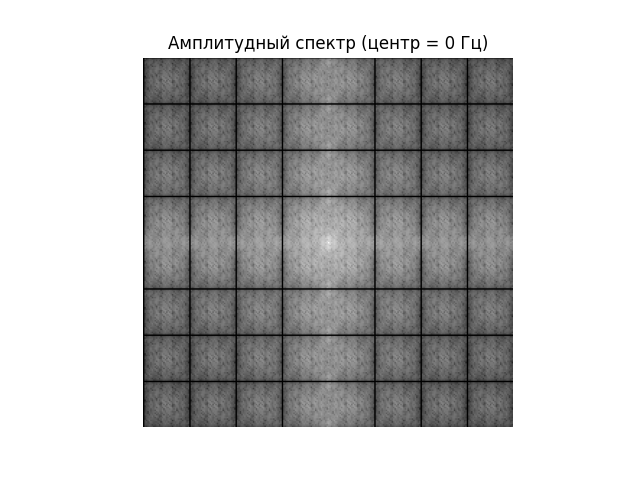
\includegraphics[width=1.0\textwidth]{images/fur_log.png}
    \caption{Логарифм модуля образа}
\end{figure}

\newpage
\subsection{Размытие по Гауссу}
Применим ядро вида
\[
\sigma = \frac{N-1}{6}
\]
\[
A_{ij} = exp \left( -\dfrac{(i-\dfrac{N+1}{2})^2 + (j-\dfrac{N+1}{2})^2}{2\sigma^2}\right) 
\]
\[
K_{\sigma} = \dfrac{A}{\Sigma_{ij}A_{ij}}
\]
Для ядер Гауссова и блочного размытия были выбраны следующие знаяения $N$: 10, 40, 120

Видно, что при $N=10$ На картинке можно различить достаточно точно, что изображено, при $N=40$ картинка ещё узнаваема, но уже трудно прочитать надпись(но если вспомнить как восстанавливают старые документы остаётся читаемой). При $N=120$ картинка уже совсем неузнаваема

% ========= ГАУССОВО ЯДРО, N=10 =========
\begin{figure}[H]
\centering
\caption{Обработка гауссовым ядром ($11\times11$)}
\label{fig:gauss_10}

% а) Исходное и обработанное (свёртка)
\begin{subfigure}[b]{0.48\textwidth}
    \centering
    
\includegraphics[width=\textwidth]{noita_gray.png}
    \subcaption{Исходное}
    \label{subfig:g10_orig}
\end{subfigure}
\hfill
\begin{subfigure}[b]{0.48\textwidth}
    \centering
    
\includegraphics[width=\textwidth]{noita_gaus10.png}
    \subcaption{Свёртка}
    \label{subfig:g10_conv}
\end{subfigure}

% б) Спектр ядра
\begin{subfigure}[b]{0.48\textwidth}
    \centering
    
\includegraphics[width=\textwidth]{ker_gaus10.png}
    \subcaption{Спектр ядра $\log|F\{h\}|$}
    \label{subfig:g10_ker_spec}
\end{subfigure}
\hfill
% в) Спектр отфильтрованного изображения
\begin{subfigure}[b]{0.48\textwidth}
    \centering
    
\includegraphics[width=\textwidth]{fur_log_filtered_gauss_10.png}
    \subcaption{Спектр результата $\log|F\{g*h\}|$}
    \label{subfig:g10_res_spec}
\end{subfigure}

% г) Сравнение методов обработки
\begin{subfigure}[b]{0.48\textwidth}
    \centering
    
\includegraphics[width=\textwidth]{noita_gaus10.png}
    \subcaption{Свёртка (scipy)}
    \label{subfig:g10_conv2d}
\end{subfigure}
\hfill
\begin{subfigure}[b]{0.48\textwidth}
    \centering
    
\includegraphics[width=\textwidth]{filtered_img_gauss_10.png}
    \subcaption{Через БПФ}
    \label{subfig:g10_fft}
\end{subfigure}

\end{figure}

% ========= ГАУССОВО ЯДРО, N=40 =========
\begin{figure}[H]
\centering
\caption{Обработка гауссовым ядром ($41\times41$)}
\label{fig:gauss_40}

% а)
\begin{subfigure}[b]{0.48\textwidth}
    \centering
    
\includegraphics[width=\textwidth]{noita_gray.png}
    \subcaption{Исходное}
\end{subfigure}
\hfill
\begin{subfigure}[b]{0.48\textwidth}
    \centering
    
\includegraphics[width=\textwidth]{noita_gaus40.png}
    \subcaption{Свёртка}
\end{subfigure}

% б)
\begin{subfigure}[b]{0.48\textwidth}
    \centering
    
\includegraphics[width=\textwidth]{ker_gaus40.png}
    \subcaption{Спектр ядра $\log|F\{h\}|$}
\end{subfigure}
\hfill
% в)
\begin{subfigure}[b]{0.48\textwidth}
    \centering
    
\includegraphics[width=\textwidth]{fur_log_filtered_gauss_40.png}
    \subcaption{Спектр результата $\log|F\{g*h\}|$}
\end{subfigure}

% г)
\begin{subfigure}[b]{0.48\textwidth}
    \centering
    
\includegraphics[width=\textwidth]{noita_gaus40.png}
    \subcaption{Свёртка (scipy)}
\end{subfigure}
\hfill
\begin{subfigure}[b]{0.48\textwidth}
    \centering
    
\includegraphics[width=\textwidth]{filtered_img_gauss_40.png}
    \subcaption{Через БПФ}
\end{subfigure}

\end{figure}

% ========= ГАУССОВО ЯДРО, N=120 =========
\begin{figure}[H]
\centering
\caption{Обработка гауссовым ядром ($121\times121$)}
\label{fig:gauss_120}

% а)
\begin{subfigure}[b]{0.48\textwidth}
    \centering
    
\includegraphics[width=\textwidth]{noita_gray.png}
    \subcaption{Исходное}
\end{subfigure}
\hfill
\begin{subfigure}[b]{0.48\textwidth}
    \centering
    
\includegraphics[width=\textwidth]{noita_gaus120.png}
    \subcaption{Свёртка}
\end{subfigure}

% б)
\begin{subfigure}[b]{0.48\textwidth}
    \centering
    
\includegraphics[width=\textwidth]{ker_gaus120.png}
    \subcaption{Спектр ядра $\log|F\{h\}|$}
\end{subfigure}
\hfill
% в)
\begin{subfigure}[b]{0.48\textwidth}
    \centering
    
\includegraphics[width=\textwidth]{fur_log_filtered_gauss_120.png}
    \subcaption{Спектр результата $\log|F\{g*h\}|$}
\end{subfigure}

% г)
\begin{subfigure}[b]{0.48\textwidth}
    \centering
    
\includegraphics[width=\textwidth]{noita_gaus120.png}
    \subcaption{Свёртка (scipy)}
\end{subfigure}
\hfill
\begin{subfigure}[b]{0.48\textwidth}
    \centering
    
\includegraphics[width=\textwidth]{filtered_img_gauss_120.png}
    \subcaption{Через БПФ}
\end{subfigure}

\end{figure}

\newpage
\subsection{Блочное размытие}
Для блочного размытия возьмём ядро вида
\[
A_{ij} = 1, \qquad K_{\square} = \dfrac{A}{\Sigma_{ij}A_{ij}}
\]

Заметим. что картинка размывается сильнее, чем размытие по гауссу, причём при $N=120$ на картинке не остаётся даже очертаний исходной картинки, а видна некотарая сетчатая структура.

% ========= БЛОЧНОЕ ЯДРО, N=10 =========
\begin{figure}[H]
\centering
\caption{Обработка блочным ядром ($11\times11$)}
\label{fig:block_10}

% а)
\begin{subfigure}[b]{0.48\textwidth}
    \centering
    
\includegraphics[width=\textwidth]{noita_gray.png}
    \subcaption{Исходное}
\end{subfigure}
\hfill
\begin{subfigure}[b]{0.48\textwidth}
    \centering
    
\includegraphics[width=\textwidth]{noita_block10.png}
    \subcaption{Свёртка}
\end{subfigure}

% б)
\begin{subfigure}[b]{0.48\textwidth}
    \centering
    
\includegraphics[width=\textwidth]{ker_block10.png}
    \subcaption{Спектр ядра $\log|F\{h\}|$}
\end{subfigure}
\hfill
% в)
\begin{subfigure}[b]{0.48\textwidth}
    \centering
    
\includegraphics[width=\textwidth]{fur_log_filtered_block_10.png}
    \subcaption{Спектр результата $\log|F\{g*h\}|$}
\end{subfigure}

% г)
\begin{subfigure}[b]{0.48\textwidth}
    \centering
    
\includegraphics[width=\textwidth]{noita_block10.png}
    \subcaption{Свёртка (scipy)}
\end{subfigure}
\hfill
\begin{subfigure}[b]{0.48\textwidth}
    \centering
    
\includegraphics[width=\textwidth]{filtered_img_block_10.png}
    \subcaption{Через БПФ}
\end{subfigure}

\end{figure}

% ========= БЛОЧНОЕ ЯДРО, N=40 =========
\begin{figure}[H]
\centering
\caption{Обработка блочным ядром ($41\times41$)}
\label{fig:block_40}

% а)
\begin{subfigure}[b]{0.48\textwidth}
    \centering
    
\includegraphics[width=\textwidth]{noita_gray.png}
    \subcaption{Исходное}
\end{subfigure}
\hfill
\begin{subfigure}[b]{0.48\textwidth}
    \centering
    
\includegraphics[width=\textwidth]{noita_block40.png}
    \subcaption{Свёртка}
\end{subfigure}

% б)
\begin{subfigure}[b]{0.48\textwidth}
    \centering
    
\includegraphics[width=\textwidth]{ker_block40.png}
    \subcaption{Спектр ядра $\log|F\{h\}|$}
\end{subfigure}
\hfill
% в)
\begin{subfigure}[b]{0.48\textwidth}
    \centering
    
\includegraphics[width=\textwidth]{fur_log_filtered_block_40.png}
    \subcaption{Спектр результата $\log|F\{g*h\}|$}
\end{subfigure}

% г)
\begin{subfigure}[b]{0.48\textwidth}
    \centering
    
\includegraphics[width=\textwidth]{noita_block40.png}
    \subcaption{Свёртка (scipy)}
\end{subfigure}
\hfill
\begin{subfigure}[b]{0.48\textwidth}
    \centering
    
\includegraphics[width=\textwidth]{filtered_img_block_40.png}
    \subcaption{Через БПФ}
\end{subfigure}

\end{figure}


% ========= БЛОЧНОЕ ЯДРО, N=120 =========
\begin{figure}[H]
\centering
\caption{Обработка блочным ядром ($121\times121$)}
\label{fig:block_120}

% а)
\begin{subfigure}[b]{0.48\textwidth}
    \centering
    
\includegraphics[width=\textwidth]{noita_gray.png}
    \subcaption{Исходное}
\end{subfigure}
\hfill
\begin{subfigure}[b]{0.48\textwidth}
    \centering
    
\includegraphics[width=\textwidth]{noita_block120.png}
    \subcaption{Свёртка}
\end{subfigure}

% б)
\begin{subfigure}[b]{0.48\textwidth}
    \centering
    
\includegraphics[width=\textwidth]{ker_block120.png}
    \subcaption{Спектр ядра $\log|F\{h\}|$}
\end{subfigure}
\hfill
% в)
\begin{subfigure}[b]{0.48\textwidth}
    \centering
    
\includegraphics[width=\textwidth]{fur_log_filtered_block_120.png}
    \subcaption{Спектр результата $\log|F\{g*h\}|$}
\end{subfigure}

% г)
\begin{subfigure}[b]{0.48\textwidth}
    \centering
    
\includegraphics[width=\textwidth]{noita_block120.png}
    \subcaption{Свёртка (scipy)}
\end{subfigure}
\hfill
\begin{subfigure}[b]{0.48\textwidth}
    \centering
    
\includegraphics[width=\textwidth]{filtered_img_block_120.png}
    \subcaption{Через БПФ}
\end{subfigure}

\end{figure}


\subsection{Ядро увеличения резкости}
Применим ядро вида
\[
K_{*} = \begin{bmatrix}
    0&-1&0\\
    -1&5&-1\\
    0&-1&0
\end{bmatrix}
\]

Видно, что на картинке выделились края пикселей.
% ========= ЯДРО ПОВЫШЕНИЯ РЕЗКОСТИ =========
\begin{figure}[H]
\centering
\caption{Обработка ядром повышения резкости $3\times3$}
\label{fig:sharp}

% а)
\begin{subfigure}[b]{0.48\textwidth}
    \centering
    
\includegraphics[width=\textwidth]{noita_gray.png}
    \subcaption{Исходное}
\end{subfigure}
\hfill
\begin{subfigure}[b]{0.48\textwidth}
    \centering
    
\includegraphics[width=\textwidth]{noita_sharp.png}
    \subcaption{Свёртка}
\end{subfigure}

% б)
\begin{subfigure}[b]{0.48\textwidth}
    \centering
    
\includegraphics[width=\textwidth]{ker_sharp.png}
    \subcaption{Спектр ядра $\log|F\{h\}|$}
\end{subfigure}
\hfill
% в)
\begin{subfigure}[b]{0.48\textwidth}
    \centering
    
\includegraphics[width=\textwidth]{fur_log_filtered_sharp.png}
    \subcaption{Спектр результата $\log|F\{g*h\}|$}
\end{subfigure}

% г)
\begin{subfigure}[b]{0.48\textwidth}
    \centering
    
\includegraphics[width=\textwidth]{noita_sharp.png}
    \subcaption{Свёртка (scipy)}
\end{subfigure}
\hfill
\begin{subfigure}[b]{0.48\textwidth}
    \centering
    
\includegraphics[width=\textwidth]{filtered_img_sharp.png}
    \subcaption{Через БПФ}
\end{subfigure}

\end{figure}

\subsection{Ядро увеличения резкости}
Применим ядро вида
\[
K_{*} = \begin{bmatrix}
    -1&-1&-1\\
    -1&8&-1\\
    -1&-1&-1
\end{bmatrix}
\]

Видно, что на картинке остались лишь очертания фигур, так как это пиксельарт информация потеряна не в большом объёме, картинка до сих пор считывается нашим глазом.

% ========= ЯДРО ВЫДЕЛЕНИЯ ГРАНИЦ =========
\begin{figure}[H]
\centering
\caption{Обработка ядром выделения границ $3\times3$}
\label{fig:edge}

% а)
\begin{subfigure}[b]{0.48\textwidth}
    \centering
    
\includegraphics[width=\textwidth]{noita_gray.png}
    \subcaption{Исходное}
\end{subfigure}
\hfill
\begin{subfigure}[b]{0.48\textwidth}
    \centering
    
\includegraphics[width=\textwidth]{noita_edges.png}
    \subcaption{Свёртка}
\end{subfigure}

% б)
\begin{subfigure}[b]{0.48\textwidth}
    \centering
    
\includegraphics[width=\textwidth]{ker_edges.png}
    \subcaption{Спектр ядра $\log|F\{h\}|$}
\end{subfigure}
\hfill
% в)
\begin{subfigure}[b]{0.48\textwidth}
    \centering
    
\includegraphics[width=\textwidth]{fur_log_filtered_edge.png}
    \subcaption{Спектр результата $\log|F\{g*h\}|$}
\end{subfigure}

% г)
\begin{subfigure}[b]{0.48\textwidth}
    \centering
    
\includegraphics[width=\textwidth]{noita_edges.png}
    \subcaption{Свёртка (scipy)}
\end{subfigure}
\hfill
\begin{subfigure}[b]{0.48\textwidth}
    \centering
    
\includegraphics[width=\textwidth]{filtered_img_edge.png}
    \subcaption{Через БПФ}
\end{subfigure}

\end{figure}

\subsection{Вывод}
Таким образом к одному и тому же изображению были применены различные ядра преобразований. Гаусовво размытие делает изображение менее чётким максимально сохраняя детали.
Блочное размытие при тех же размерах матрицы размывает изображение сильнее и не сохраняет детали. При увеличении размера матрицы оба размытия работаю сильнее.
Применение ядер повышения резкости и выделения краёв действуют в соответствии со своими названиями.
Изображения после фильтрации через conv2 и через БПФ работает немного по разному, это происходит из-за того, что в conv2 используется линейная свёртка, а свёртка через БПФ работает как циклическая свёртка.


\end{document}
